\chapter{Analysis}
\label{analysis}

The analysis consists of multiple steps, that will be explained in the following.
All parameters for the analysis as well as the features used for the
different Random Forests can be found in the appendix \ref{sec:app_params}.

\section{Simulated Data and Preprocessing}
% configuration in appendix! + algorithmen beim prep

\subsection{Monte Carlo Data}
Our analysis is based entirely on simulated Monte Carlo (MC) data.
The particle shower simulation is done with the software CORSIKA \cite{heck1998corsika}, 
the simulation of the instrument response goes by the name of SIMTEL \cite{BERNLOHR2008149}.

Monte carlo data is simulated and shared across the CTA collaboration, 
our analysis uses the data from the PROD3 simulation of 
the CTA south array. These simulation include more telescopes 
than the array will eventually have. This is done to compare
different layouts and telescope positions.
We will choose the relevant telescopes in a way, that
our array resembles the earlier mentioned south array (See section \ref{sec:cta}).

The CORSIKA simulations start with particles of a given energy that hit the atmosphere,
propagate through the air and arrive at the telescopes locations.
The SIMTEL-simulations include the array layout, instrument response and trigger settings to
evaluate if and how an event is going to be recorded.

Our data contains everything the telescopes would measure
at a low level
plus additional MC information, that will not be present at real experiments.
This includes the simulated particle direction, energy and type.
This ground-truth or MC-truth allows us to gauge the effectiveness of our 
algorithms by comparing the predictions with the MC-truth values.

% The total number of simulated data after the low level analysis 
% is shown in table \ref{tab:mc_infos}.

% \begin{table}
%     \caption{Take the infos from the simtel files instead! List file sizes aswell}
%     \begin{center}
%         \begin{tabular}{l r r r}
%             \hline
%             & Pointlike Gamma & Diffuse Gamma & Protons \\
%             %\hline
%             MC runs & \num{1113} & \num{17382} &  \num{9273} \\ 
%             %\hline
%             Array events & \num{955317} & \num{3409290} & \num{4657529} \\
%             %\hline
%             Telescope events & \num{4554313} & \num{14383270} & \num{20106385} \\
%             %\hline
%             Accumulated file sizes & 0 & 0 & 0 \\
%         \end{tabular}
%     \end{center}
%     \label{tab:mc_infos}
% \end{table}

At the lowest available level our "observed" data consists of uncalibrated waveforms 
in the camera pixels.
We will perform several analysis steps that would also be needed for real data.
The choice of parameters for the low level processing 
is based on values from earlier studies, such as \cite{kai_diss}.

To adress a specific event, we will split the event information into
three layers, that will be saved as separate dataframes, denoted with the keys:
\begin{enumerate}
    \item{$run$: This contains non-event-specific information about the monte carlo run, e.g.
    spectral\_index, particle injection height, ...}
    \item{$array\_events$: Any shower that triggered the array at some point 
    is considered to be an array event.
    Array-level features consist of array-wide shared event information 
    (e.g. number of triggered telescopes, average intensity),
    reconstructed high-level features of the primary particle (e.g. energy, source position) and the 
    event specific monte carlo information to compare the reconstructed values against.}
    \item{$telescope\_events$: This includes how a specific telescope has seen the shower and
    contains information about the telescope itself (e.g. focal length). Telescope-level features 
    describe the camera image and contain reconstructed features that were retrieved based on 
    the telescope's specific measurements.}
\end{enumerate}
In the following we will 
distinguish between "array-events" and "telescope-events" when describing the reconstruction methods
with available information as mentioned above.
The number of triggered telescopes in an array-event 
will be referred to as the event multiplicity.

\subsection{Reconstruction on Telescope Tevel}
\label{sec:tel_analysis}

To be able to apply high-level analysis methods, the initial data 
needs to be reduced and processed substantially.

Processing of the simtel-files is done with the aforementioned ctapipe, starting with 
the calibration of the event. The calibration performs an integration of the waveforms in 
each pixel of a triggered telescopes camera. 
This reduces the waveforms to two values per pixel: An integrated value which describes 
the amount of light captured during the pulse and a peak value indicating the 
(relative) arrival time of the measured pulse. These are referred to as 
photo-electron equivalents (phe) and pulse time in the following.
Inside of ctapipe the initial data is referred to as R1
and the resulting data after the integration as dl1.

The resulting images get cleaned with a tailcuts approach before they are
used to calculate image features, such as the hillas parameters.
The tailcuts cleaning is a two-step method based on the pixel value:
First, all pixels with a value below an upper threshold get discarded from 
the image. Second, all discarded pixels above a lower threshold, that also 
happen to have at least a fixed amount of neighbouring pixels surviving the first step,
get added back in.
Another cleaning method, that also includes the arrival time information, 
was implemented and tested, but did not lead to any better results in this
specific analysis.
To keep the analysis more comparable to other works, we stayed with 
the tailcuts cleaning algorithm, which was the default algorithm at the time 
of this analysis.

After the image is cleaned, image features get calculated.
This includes the classic hillas parameters among others.
In total we calculate the following parameters:

\textbf{Hillas Parameters:}

These provide a general, basic description of the image 
in camera coordinates and form the base for 
all subsequent analyses. Calculation is performed with a
principal component analysis. The semi-major axis of the ellipse
will be referenced as main shower axis.

\begin{itemize}
    \item{$x, y$: Coordinates of the image cog}
    \item{$r, \phi$: Coordinates of the cog in polar coordinates}
    \item{$intensity$: Sum of photo-electrons across all pixels}
    \item{$length, width$: Size of the image ellipse}
    \item{$\psi$: Angle between ellipse orientation and x-axis}
    \item{$skewness, kurtosis$: Higher order image moments along the shower axis}
\end{itemize}

\textbf{Leakage:}

These describe how much of the shower was captured by the camera.
A lot of information at the edge of the camera indicates, that part of the light missed the telescope, 
which makes the reconstruction less reliable.
Besides, this information is important to estimate the primary energy.

\begin{itemize}
    \item{$leakage\_1\_intensity$: Percentage of photo-electrons in the outer most ring of pixels with respect to the photo-electrons in the whole image}
    \item{$leakage\_1\_pixel$: Percentage of pixels in the outer most ring of pixels with respect to the pixels in the whole image}
    \item{$leakage\_2\_intensity$: Percentage of photo-electrons in the two outer most rings of pixels with respect to the photo-electrons in the whole image}
    \item{$leakage\_2\_pixel$: Percentage of pixels in the two outer most rings of pixels with respect to the pixels in the whole image}
\end{itemize}

\textbf{Concentration:}

These describe how constrained the light distribution is.
\begin{itemize}
    \item{$concentration\_cog$: Percentage of photo-electrons in the three pixels closest to the cog with respect to the photo-electrons in the whole image}
    \item{$concentration\_core$: Percentage of photo-electrons inside the hillas ellipse with respect to the photo-electrons in the whole image}
    \item{$concentration\_pixel$: Percentage of photo-electrons in the brightest pixel with respect to the photo-electrons in the whole image}
\end{itemize}

\textbf{Timing Information:}

These describe the temporal evolution of the captured light.
This can be useful to improve the reconstruction of the source position.
\begin{itemize}
    \item{$slope, slope\_err$: Slope and corresponding  error of a linear regression to the pixel-wise pulse times along the main shower axis.}
    \item{$intercept, intercep\_err$: Intercept and corresponding  error of a linear regression to the pixel-wise pulse times along the main shower axis.}
    \item{$deviation$: Root-mean-square deviation between the individual pulse times and the pulse times
        retrieved via the linear regression at the cog.}
\end{itemize}

\textbf{Other:}

The way clusters form in the image can give hints towards the classification of the primary particle.
\begin{itemize}
    \item{$num\_islands$: Number of individual clusters in the cleaned image.}
    \item{$num\_pixel\_in\_shower$: Number of pixels that survived the cleaning.}
\end{itemize}

All these features get used in the machine learning algorithms at later stages.

\subsection{Hillas Reconstructor}  % we dont seperate between 0 and 1 right?
After the image processing of each associated telescope image has been finished,
the predictions of our "benchmark" source position estimator get calculated.
This algorithm is referred to as HillasReconstructor inside ctapipe, because 
it works based on the hillas parametrisations of the images.

For each triggered telescope, a 2D-plane is drawn into the spatial 3D-space based on the main shower 
axis and the telescope orientation. These planes intersect and 
the weighted average of all intersections yields the 
main interaction point of the observed shower ($h_{max}$).
Intersecting the main shower axes on the ground frame leads to 
an estimation of the impact point on the ground ($core$).
For a general illustration see figure \ref{fig:hillas_reconstructor}.

Together these can be used to reconstruct the shower origin.
Right now this is the default reconstruction algorithm inside ctapipe.
The current implementation does not provide an 
estimation for the uncertainty of the reconstructed parameters.

\begin{figure}
	\centering
	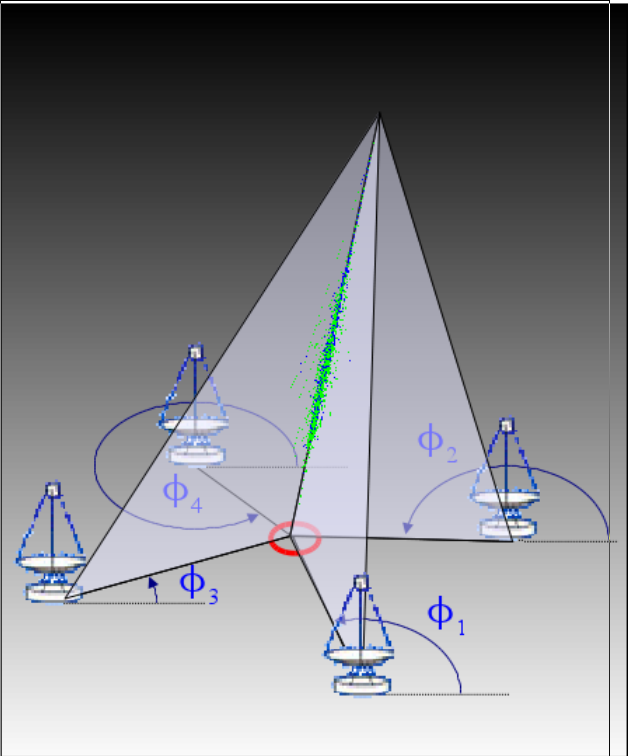
\includegraphics[width=0.6\textwidth]{images/hillas_reco.png}
	\caption{Illustration of a stereoscopic reconstruction of the source position.
    From each telescope a plane is drawn, the direct intersection 
    on the ground leads to the impact point (red circle).
    The image is taken from a habilitation thesis by 
    Mathieu de Naurois \cite{hillas_reco}.
    Not included is the reconstruction of the main interaction point,
    that could be obtained by calculating a weighted average of the plane
    intersections.}
	\label{fig:hillas_reconstructor}
\end{figure}

Since this method inherently requires a stereoscopic experiment
and multiple triggered telescopes, it will not work for a single telescope.

In total, this step leads to the following features on array level:
\begin{itemize}
    \item{$alt, az$: Reconstructed source position}
    \item{$core\_x, core\_y$: Reconstructed core position on the ground}
    \item{$average\_intensity$: Mean intensity over all triggered telescopes}
    \item{$h\_max$: Reconstructed main interaction height}
\end{itemize}

\section{High Level Analysis}

High level analysis of the preprocessed data is based on the use of
the aict-tools package \cite{aict-tools} which itself makes use of
sklearn \cite{sklearn_api} for the implementation of the machine learning algorithms.
The aict-tools have originally been developed for the FACT-experiment
which is a single IACT. 
For this reason
adaptions had to be made compared to the status of the project at the start 
of this thesis to perform a stereoscopic analysis.

The algorithm of choice is the random forest algorithm.
Model feature importance will be calculated
based on the sklearn functionality, which
uses the mean decrease impurity.
For a discussion on feature importance estimations see \cite{hastie2017springer}.
As we use the feature importance as a mere sanity check for our algorithms 
and not base the analysis on them, we will settle with the available method.
Separate models are trained for the tasks of gamma/hadron
separation and signal source position reconstruction.

The size of the available data after the earlier 
preprocessing steps is summarized in table \ref{tab:events_after_prep}.


\begin{table}
    \caption{Number of remaining events for each simulated particle type after the
    preprocessing. Pointlike gammas get used for the evaluation, diffuse gammas and protons
    get used for the training of the models. In order to optimize the models not all
    available data gets used.}
    \begin{center}
        \begin{tabular}{l r r r}
            %\hline
            & Pointlike Gamma & Diffuse Gamma & Protons \\
            \hline
            MC runs & \num{1113} & \num{17382} &  \num{9273} \\ 
            %\hline
            Array events & \num{955317} & \num{3409290} & \num{4657529} \\
            %\hline
            Telescope events & \num{4554313} & \num{14383270} & \num{20106385} \\
            %\hline
        \end{tabular}
    \end{center}
    \label{tab:events_after_prep}
\end{table}

To achieve more robust models and avoid overfitting, the data gets split into mutiple dataframes.
The gamma-/hadron-separation model and the DISP-/SIGN-models each get 
40\% of the available diffuse gamma data for training. 20\% are left out
as a test dataframe for sanity checks.

We only use 30\% of the proton events to have a roughly even class distribution while training 
the gamma-/hadron-separation model.

The pointlike gamma events are not used for the training of the models,
but only to evaluate the models later.
For this all available data gets used.

\subsection{Gamma-/Hadron-Separation}
\label{sec:gh_sep}

For the task of gamma/hadron separation a random forest will be trained
on telescope-event level with the features from \ref{sec:measuring}.
The random forest is set to predict a class probability instead of
the class itself. 
In addition the features from the earlier
HillasReconstructor step were added.
Performance of the Classifier will be gauged based 
on the area under the receiver-operating-charateristic curve (AUC).
Selecting a threshold for classification will be based on
the $F_{\beta}$-score with $\beta = 0.1$.
Adding the additional features is not necessary, but was found to improve
the AUC by a few percent.

The single telescope predictions will be combined by
taking the mean of the single
single predictions to provide a prediction for the complete
array-event.


% \section{energy estimation}
% Energy estimation can be performed in the same way as the gamma/hadron
% separation. For this task there has been earlier work indicating
% the usefulness of a second machine learning model trained
% on the predictions of the first telesope-level model
% \cite{ba-lars}.

% I am thus going to present results based on either calculating the mean
% of the telescope level predictions and using a second random forest
% to improve the array level prediction.

\subsection{Reconstruction of the Source Position}
\label{sec:source_position}

The position on the shower axis can be estimated based on 
the hillas parameters and other image features, as 
explained in section \ref{sec:measuring}.

The calculation of the DISP is based on all the image-level
features listed in \ref{sec:tel_analysis}.
In this case this is done using a Random Forest.
At this point the reconstructed source position
is fixed at two points at the main shower axis.

To resolve the head/tail ambiguity in monoskopic mode,
we will train a second random forest.
This is referred to as SIGN-prediction, interpreting the two possible sides
as $\pm1$, allowing for binary classification.
Using a second Random Forest is also done in FACT-analyses,
where stereoscopic information are not available \cite{fact_sign_performance}.
The monoscopic prediction is then the chosen point in camera coordinates transformed
to sky coordinates (alt/az).
% In our case this is only needed to provide baseline predictions
% on telescope level.
Our simple baseline estimation for the stereoscopic reconstruction will 
calculate the median in alt/az of the single predictions.

Additionaly we employ an approach inspired by 
what the MAGIC-collaboration does in some of their analyses.
In the case of the MAGIC-telescopes the ambiguity does not
get resolved until the individual results get combined
on the stereo level. The choice of the correct
pair out of the four reconstructed positions can be done either
by calculating the crossing point of both main shower axises
or by calculating the pairwise distances between the positions \cite{ALEKSIC201676}.
In MAGIC events where the minimum distance between two points is larger than a set threshold
get discarded.

The method, where all four distances get calculated, is illustrated in figure \ref{fig:disp_magic}

\begin{figure}
    \centering
    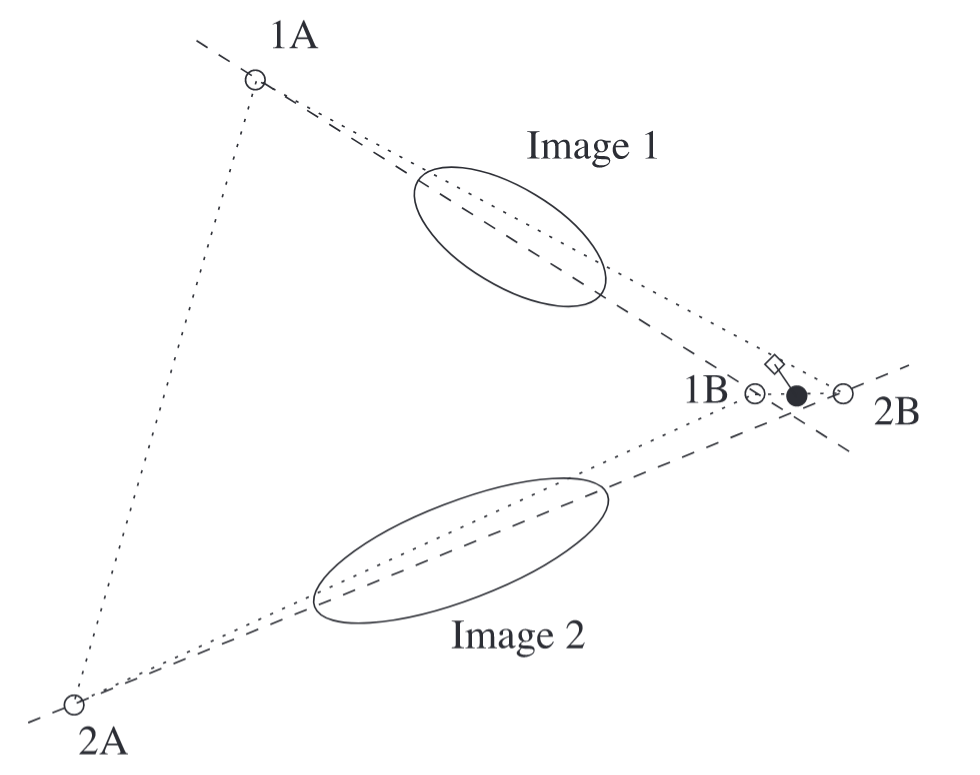
\includegraphics[width=0.8\textwidth]{images/magic_stereo_disp.png}
    \caption{Illustration of the stereoscopic DISP-reconstruction used in MAGIC.
        Two shower ellipses are drawn with the respective main shower axes as dashed lines
        and the two disp predictions each marked as 1A, 1B, 2A, 2B.
        The pairwise distances are displayed by the dotted lines.
        The closest pair is 1B-2B, the resulting prediction is calculated as 
        weighted average between the two points. The true source position is marked with a diamond.
        The illustration has been taken from a study of the Crab Nebula with MAGIC,
        showing the effect of extensive upgrades in 2011-2012 \cite{ALEKSIC201676}.}
    \label{fig:disp_magic}
\end{figure}

Since we have more than 2 telescopes in CTA and 
a variable number of triggered telescopes per array-event,
we need to adapt this method in a scalable way.

The most obvious approach seemed to be an iterative one:
For each pair of triggered telescopes, we combine the results 
in the way described above. In fact we forgo the part where events get discarded 
if the minimum distance is too big. This is done to keep the same event count to
compare the results to the HillasReconstructor without accidentially creating a bias in the dataset.
At the same time the choice of a specific threshold does not seem obvious
with different telescopes and event multiplicities.
Figure \ref{fig:stereo_disp} illustrates this method for the case of 4 triggered telescopes.

From our research it seemed to have little to no effect to weight
the average of the two points based on common image features such as 
the intensity or size.

We then save all intermediate results and average them to get the final prediction.
In this case taking the median of the pairwise predictions seemed to be more robust
than the mean, weighted or unweighted.

\begin{figure}
    \centering
    \begin{subfigure}{0.45\textwidth}
        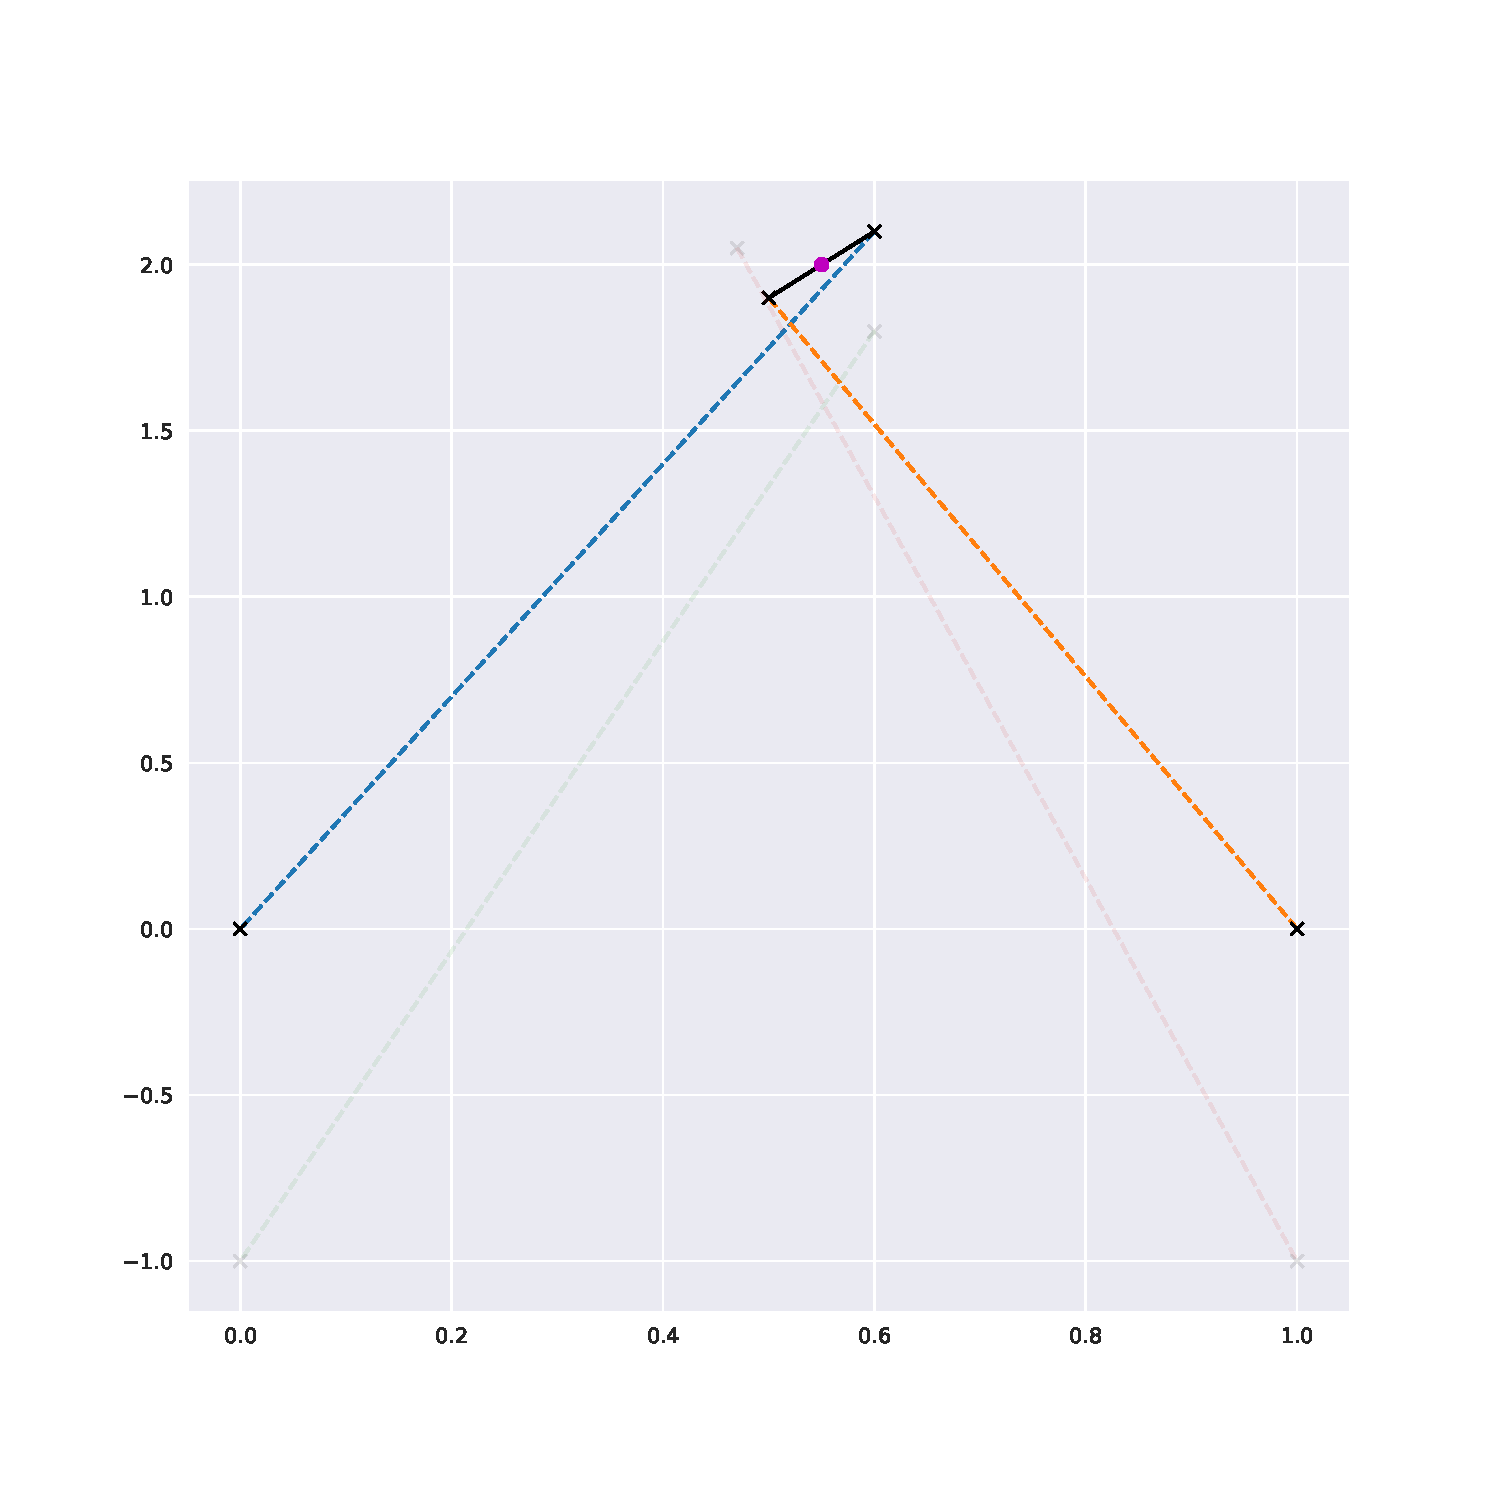
\includegraphics[width=0.8\linewidth]{Plots/stereo_magic_1.pdf}
        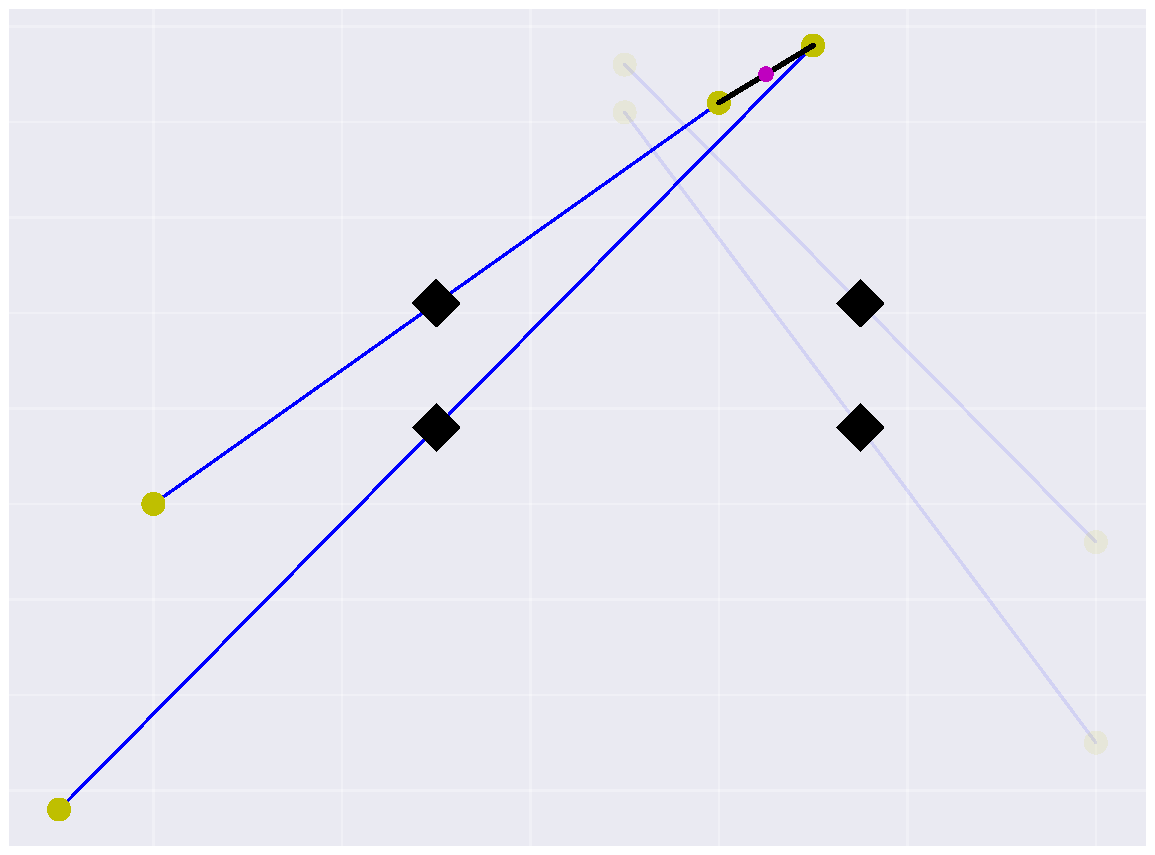
\includegraphics[width=0.8\linewidth]{Plots/stereo_magic_2.pdf}
        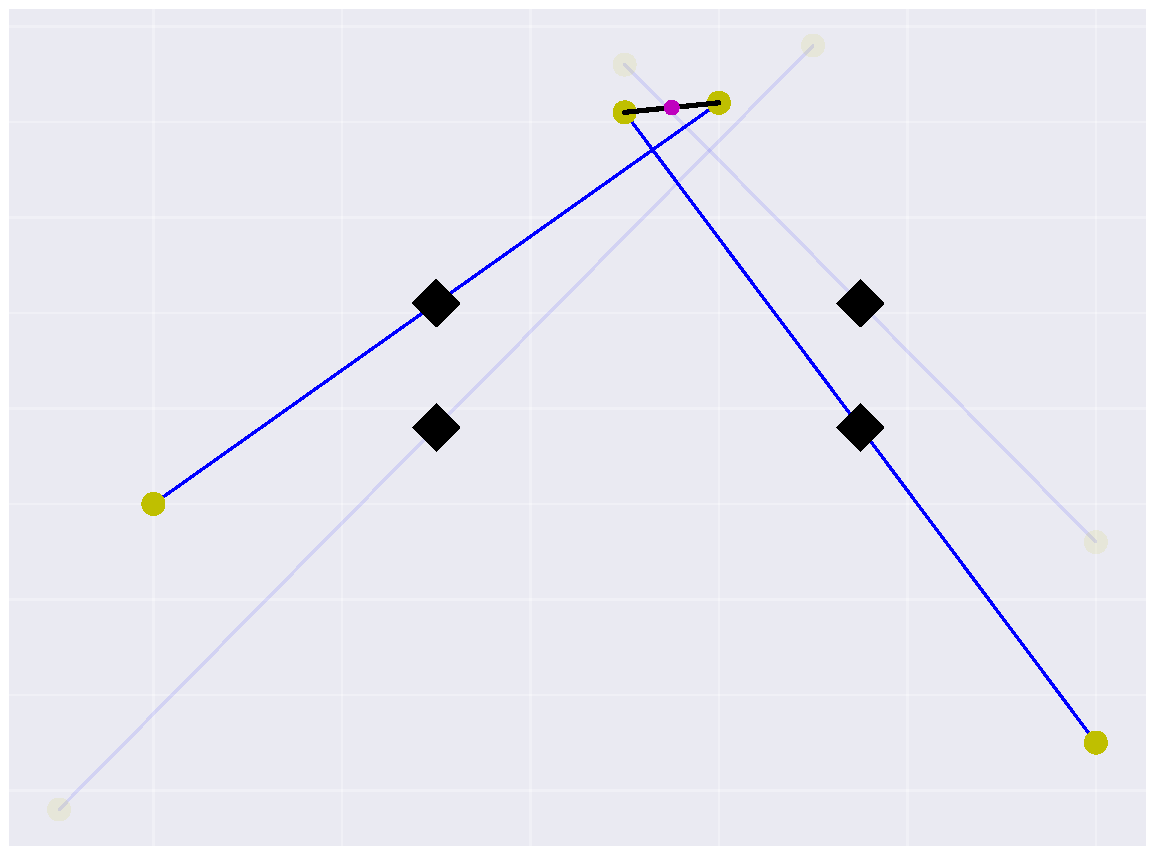
\includegraphics[width=0.8\linewidth]{Plots/stereo_magic_3.pdf}
    \end{subfigure}
    \begin{subfigure}{0.45\textwidth}
        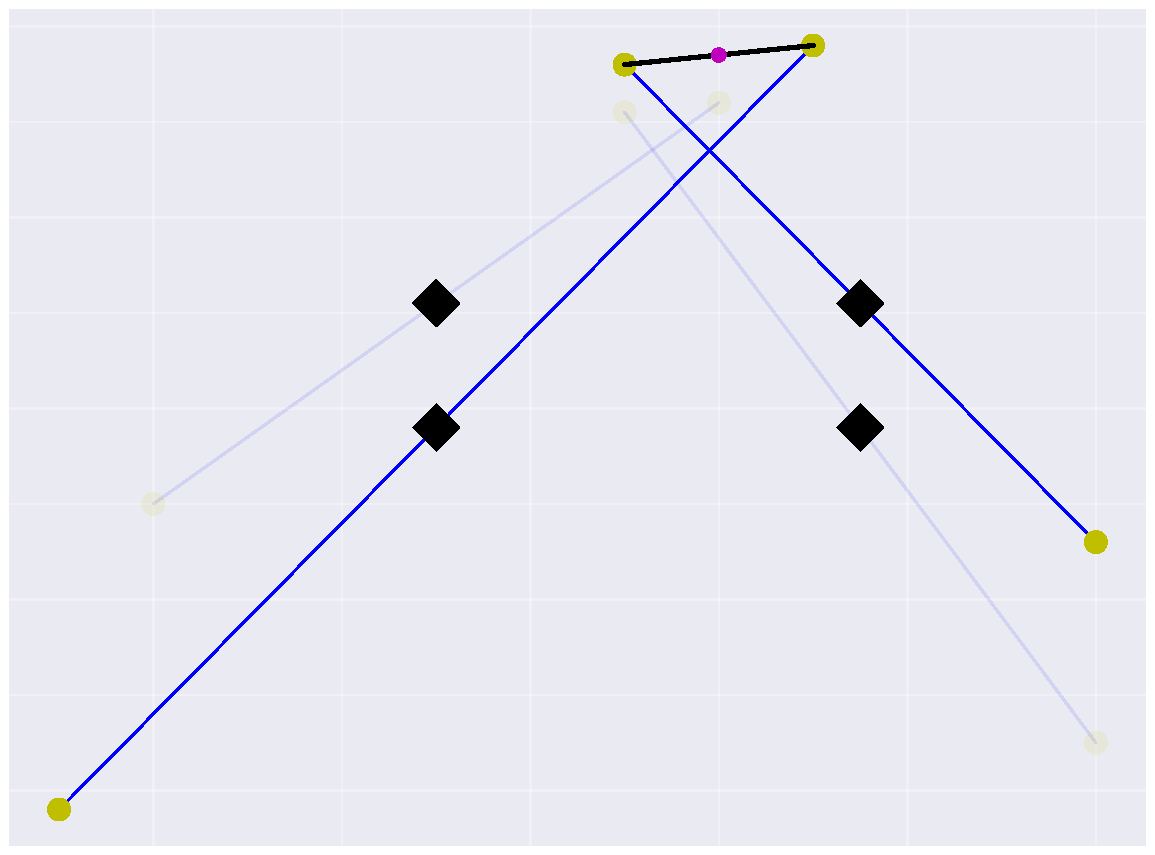
\includegraphics[width=0.8\linewidth]{Plots/stereo_magic_4.pdf}
        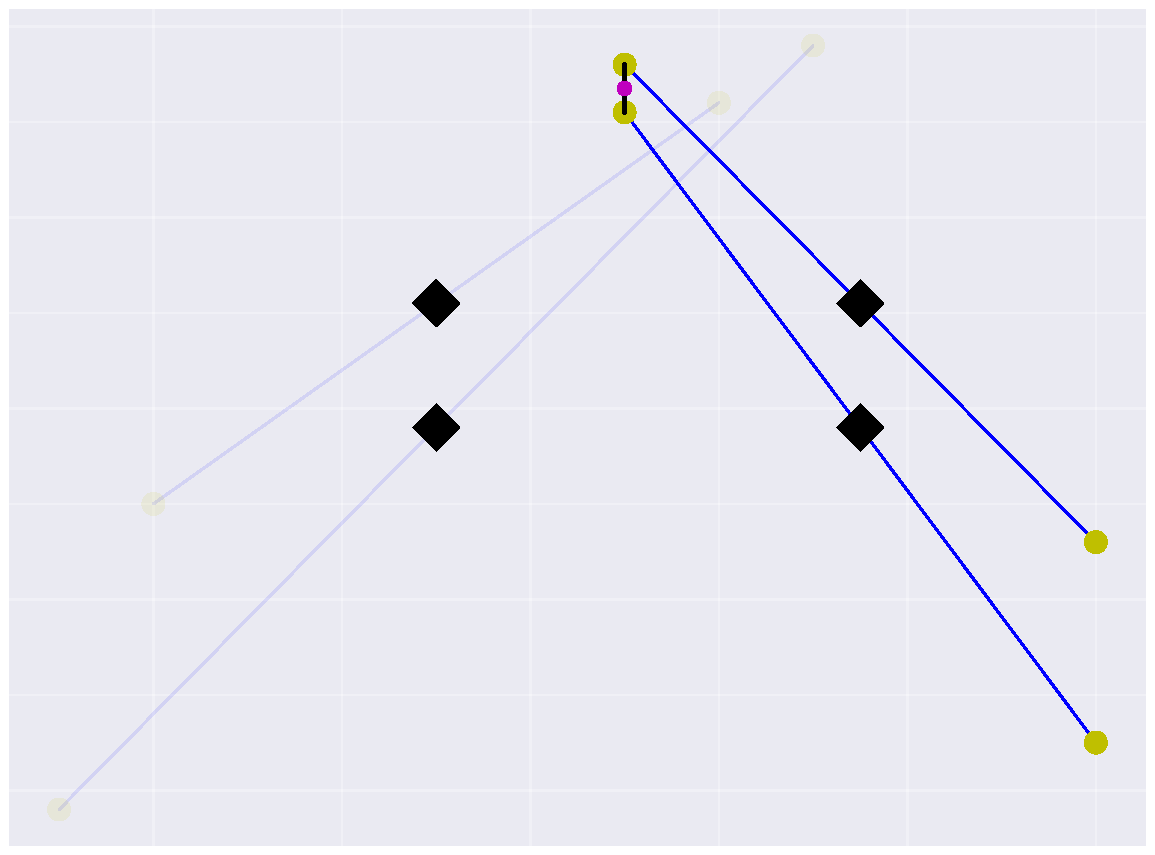
\includegraphics[width=0.8\linewidth]{Plots/stereo_magic_5.pdf} 
        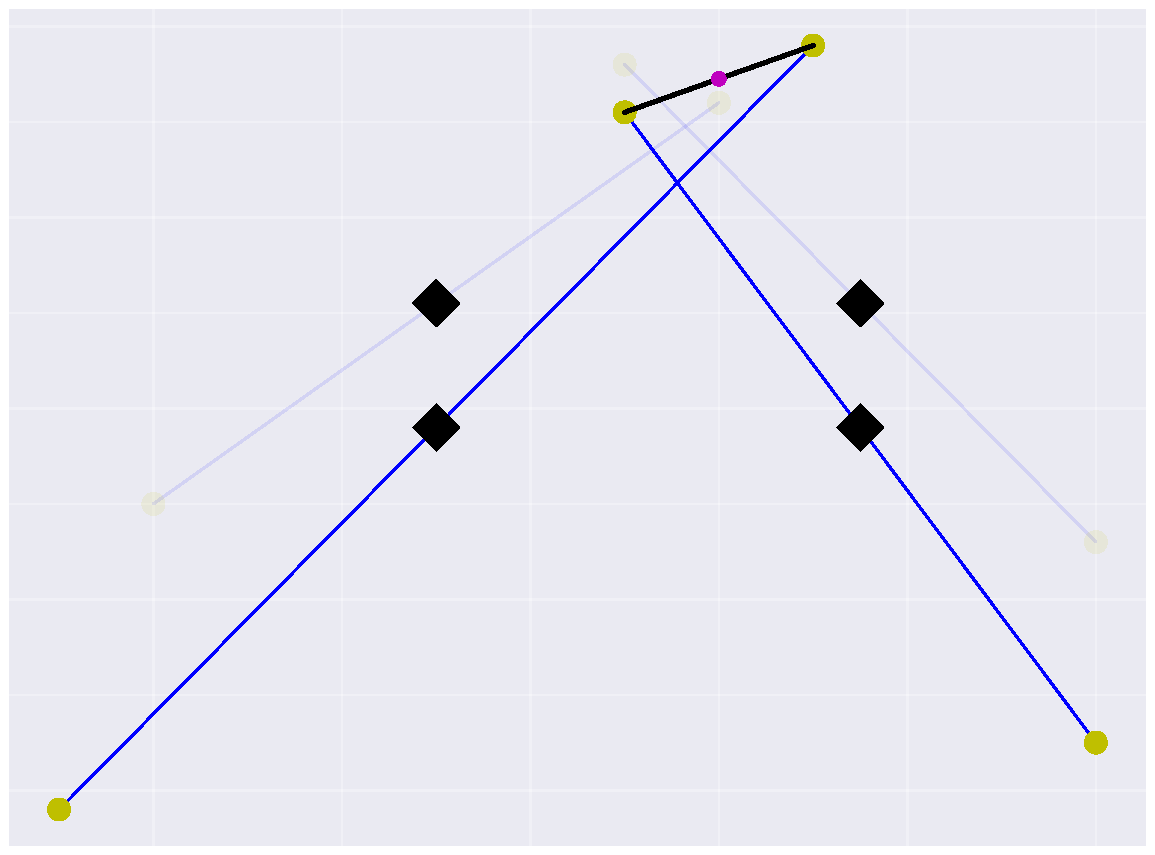
\includegraphics[width=0.8\linewidth]{Plots/stereo_magic_6.pdf} 
    \end{subfigure}
    \caption{
    Illustration of the iterative extension to the stereoscopic magic approach
    with the DISP-predictions as unfilled dots, the intermediate resulting prediction
    as filled dot and the true source position as unfilled diamond.
    Four telescopes have triggered, leading to a total of eight individual DISP-predictions.
    For each pair of telescopes, the four predictions get evaluated according to \cite{ALEKSIC201676}
    without dismissing poor events based on the minimum distance, leading to one 
    intermediate prediction per unique pair.
    Averaging the six intermediate results leads to the final prediction.}
    \label{fig:stereo_disp}
\end{figure}

\iffalse
\section{Analysis for a single LST}
Inspired by the current status of CTA with only one LST operating and no MSTs or SSTs
on the north side just yet,
we wanted to add a completely monoskopic analysis.

This is in fact not a real monoscopic analysis and not performed on the north 
side as well. It is merely meant to show that the DISp+SIGn approach works as
expected for the monoscopic LST case.

(MEHR TELESKOPE?? VOLLES MODELL? ALLGEMEIN ALLES NOCH ZIEMLICH WHACKY HIER)
For this reason we chose a single telescope of the simulated data.
Choosing multiple telescopes and treating them as independent events 
would most likely be a valid option as well, although the 
events would not be 100\% uncorellated.

We perform the same analysis for this reduced dataset, leaving out only 
the stereoscopic parts of the analysis.
The machine learning models are expected 
to perform slightly worse as the stereoscopic features are missing.

As explained the HillasReconstructor does not work on a single telescope.
The only source-position predictions we can make and compare are monoscopic 
DISP+SIGN-predictions with the MC truth.
\fi